\begin{frame}
	\frametitle{Integrated Design}
	Non-operating Reactor Site + Borehole Repository
	\begin{itemize}
		\item Save cost on decommissioning (some parts)
		\item Earn Revenue from hosting repository
		\item Save cost on repository facility construction
			  with already existing infrastructure
		\item Communities that benefit from power plants are more likely
			  to be friendly
	\end{itemize}
\end{frame}

\begin{frame}
	\frametitle{Why Boreholes?}
	\begin{itemize}
		\item Less rigorous geolgoical standard (flexible siting)
		\item modularity
		\item Area(30$km^2$ for 70,000MTHM)
		\item Less Cost
	\end{itemize}
	\begin{figure}[htbp!]
		\begin{center}
			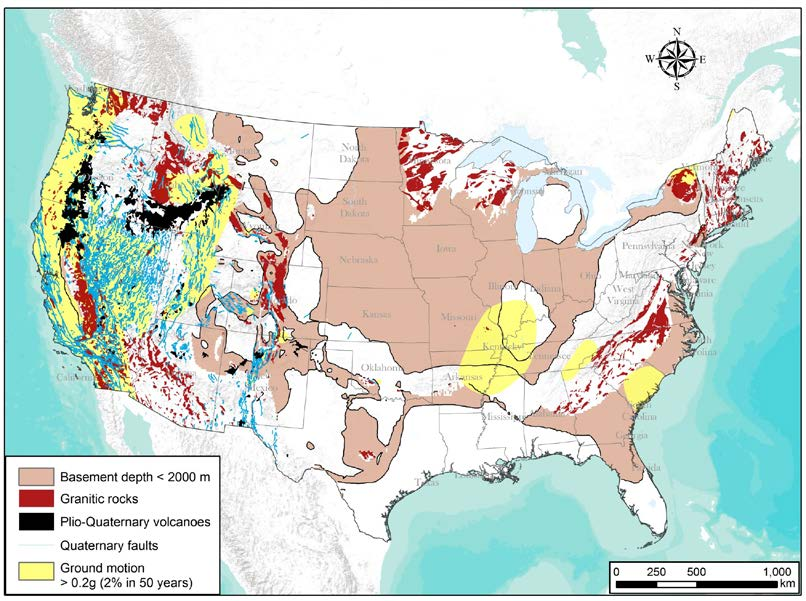
\includegraphics[height=4cm]{./images/cbrock.png}
		\end{center}
		\caption{Map of Areas in US with crystalline basement rock at less than 2,000m in depth.
			Pink areas are suitable for a borehole repository.
			 \cite{freeze_siting_2015}.}
		\label{fig:basement_map}
	\end{figure}
\end{frame}

\begin{frame}
	\frametitle{Method of Comparison: Case Study}
	Two cases:
	\begin{itemize}
		\item Reference/Base Case: Yucca Mountain
		\item Proposed Case: Borehole Repository at Clinton Power Station (Clinton, IL)
	\end{itemize}
\end{frame}

\begin{frame}
	\frametitle{Why Clinton?}
	\begin{itemize}
		\item Clinton is under risk of shutting down, despite the recent bill that saved
		it from shutting down. (Inherent economic disadvantage of single - unit reactor site)
		\item Geological study done for Decatur Carbon Sequestration Project
		\item Socio-Economic research done in impacts of its shutdown
		\item Central Location (low MTHM*km value)
	\end{itemize}
\end{frame}

\begin{frame}
	\frametitle{6 Quantitative Metrics}
	\begin{itemize}
			\item Transportation Burden $[MTHM \cdot km]$: Less SNF to be transported
			\item Workforce Utilization $[-]$: Pre existing skilled workforce
			\item Expediency $[y]$: Faster the removal of SNF, more cost savings
			\item Consent Basis $[\frac{nuclear MW}{\mbox{capita}}]$: More familiarity
			and dependency to nuclear = more likely to be consenting
			\item Site Access $[-]$: Rail access to the site is essential for 
			beginning operations.
			\item Site Appropriateness $[-]$: Must be geologically viable.
	\end{itemize}

\end{frame}

\begin{frame}
	\frametitle{Stakeholders}
	\begin{itemize}
		\item the federal government,
		\item the state government,
		\item the local government / community,
		\item and the owner of the non-operating plant.
	\end{itemize}
\end{frame}


\begin{frame}
	\frametitle{Evaluation Method}
	For Each Metric:
	\begin{align} 
		\mbox{NV} &= \frac{x-\mbox{W}}{\mbox{B}-\mbox{W}}\\
		NV &= \mbox{normalized value for the metric}\\
		x &= \mbox{considered case value for the metric}\\
		B &= \mbox{best case value for the metric}\\
		W &= \mbox{worst case value for the metric}\\
	\end{align}
	Some are Boolean - either yes or no.
\end{frame}

\begin{frame}
	\frametitle{Stakeholder Weights}
	Weight of metric for each Stakeholder is up to the discretion of evaluator's interpretation.
	For this paper, the following weight is used:
	\begin{table}[h]
		\centering
		\caption {Metrics and Weight for Each Stakeholder}
		\label{tab:stakeholders_weight}
		\scalebox{0.8}{
			\begin{tabular}{|l|c|c|c|c|}
				\hline
				Metric & Federal & State & Local & Utility  \\ \hline
				Transportation Burden & 3 & 2 & 1 & 1    \\ \hline
				Site Appropriateness & 3 & 2 & 1 & 1 \\ \hline
				Workforce Utilization & 3 & 2 & 2 & 2 \\ \hline
				Consenting Locals & 3 & 2 & 3 & 2 \\ \hline
				Site Access & 3 & 2 & 1 & 1 \\ \hline
				Expediency & 3 & 2 & 1 & 3 \\ \hline \hline
			\end{tabular}}
		\end{table}
	\end{frame}